\documentclass{article}

\usepackage[T1]{fontenc}
\usepackage[polish]{babel}
\usepackage{geometry}
\usepackage{graphicx}

\title{
  \huge \textbf{Projekt 1 - Mnożenie macierzy}\\~\\
  \LARGE Temat 2 - Dla macierzy o rozmiarze mniejszym lub równym $2^l \times 2^l$ algorytm tradycyjny. Dla macierzy o
rozmiarze większym od $2^l \times 2^l$ algorytm rekurencyjny Strassena.}
\author{Bartłomiej Jamiołkowski, Cyprian Neugebauer}
\date{March 14, 2024}

\begin{document}
\maketitle

\section{Pseudokod}

\subsection{Kod wyboru algorytmu na podstawie parametru l}
Podstawową ideą naszego programu jest wybór algorytmu w zależności od rozmiaru macierzy. Dla macierzy o rozmiarze
mniejszym lub równym $2^l \times 2^l$ wykonywany jest algorytm tradycyjny, w przeciwnym
razie wykonywany jest algorytm Strassena.

\begin{figure}[h]
  \centering
  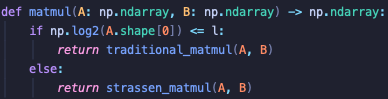
\includegraphics[width=0.9\textwidth]{matmul.png}
  \caption{Kod wyboru algorytmu na podstawie parametru l}
\end{figure}
\newpage

\subsection{Tradycyjny algortym mnożenia macierzy}

W implementacji tradycyjnego mnożenia macierzy wykonujemy następujące kroki:
\begin{enumerate}
    \item Tworzymy pustą macierz wynikową $C$ o wymiarach odpowiadających liczbie wierszy macierzy $A$ i liczbie kolumn macierzy $B$, aby przechowywać wyniki operacji.
    \item Rozpoczynamy proces mnożenia od iteracji przez wszystkie wiersze macierzy $A$. 
    \item Dla każdego wiersza z macierzy $A$ przeprowadzamy iterację po wszystkich kolumnach macierzy $B$.
    \item Dla każdej pary (wiersz z $A$, kolumna z $B$):
    \begin{enumerate}
        \item Mnożymy odpowiadające sobie elementy z wiersza macierzy $A$ i kolumny macierzy $B$.
        \item Sumujemy wyniki tych mnożeń.
    \end{enumerate}
    \item Zapisujemy wynik sumy w macierzy $C$ na pozycji odpowiadającej wierszowi z macierzy $A$ i kolumnie z macierzy $B$. Dla $i$-tego wiersza macierzy $A$ i $j$-tej kolumny macierzy $B$, wynik zapisujemy na pozycji $C[i, j]$.
\end{enumerate}

\begin{figure}[h]
  \centering
  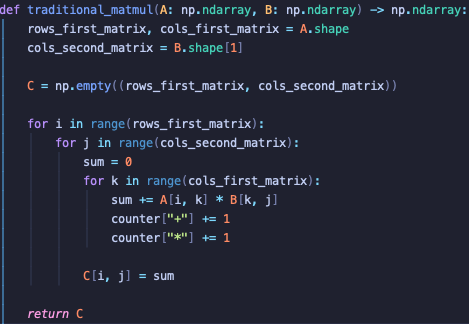
\includegraphics[width=0.9\textwidth]{traditional_matmul.png}
  \caption{Kod tradycyjnego algorytmu mnożenia macierzy}
\end{figure}

\subsection{Algorytm rekurencyjny Strassena}

Algorytm Strassena do mnożenia macierzy jest metodą, która pozwala na redukcję liczby operacji mnożenia przez
rekurencyjny podział macierzy i zastosowanie specjalnych kombinacji sum i różnic ich podmacierzy.

\begin{enumerate}
    \item \textbf{Warunek bazowy:} Gdy macierz ma wymiar $1 \times 1$, elementy $A$ i $B$ są mnożone bezpośrednio, a wynik jest zwracany.
    \item \textbf{Podział macierzy:} Macierz $A$ i $B$ jest dzielona na cztery podmacierze: $A_{11}, A_{12}, A_{21}, A_{22}$ dla $A$ oraz $B_{11}, B_{12}, B_{21}, B_{22}$ dla $B$.
    \item \textbf{Obliczanie produktów pomocniczych:} Za pomocą określonych kombinacji podmacierzy $A$ i $B$, obliczane jest siedem produktów pomocniczych $P_1$ do $P_7$.
    \item \textbf{Konstrukcja macierzy wynikowej $C$:} Korzystając z operacji dodawania i odejmowania na produktach $P_1$ do $P_7$, formowane są cztery podmacierze wynikowe $C_{11}, C_{12}, C_{21}, C_{22}$.
    \item \textbf{Łączenie podmacierzy w macierz wynikową:} Z podmacierzy $C_{11}, C_{12}, C_{21}, C_{22}$ składana jest pełna macierz wynikowa $C$, przy użyciu funkcji \texttt{np.block}.
\end{enumerate}

\begin{figure}[h]
  \centering
  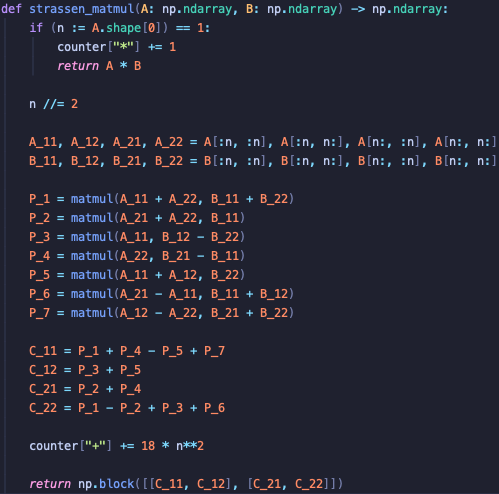
\includegraphics[scale=0.59]{strassen_matmul.png}
  \caption{Kod mnożenia macierzy algortymem Strassena}
\end{figure}

\section{Wykresy}

\subsection{Wykresy czasu mnożenia macierzy dla różnych $l$}

\begin{figure}[h]
  \centering
  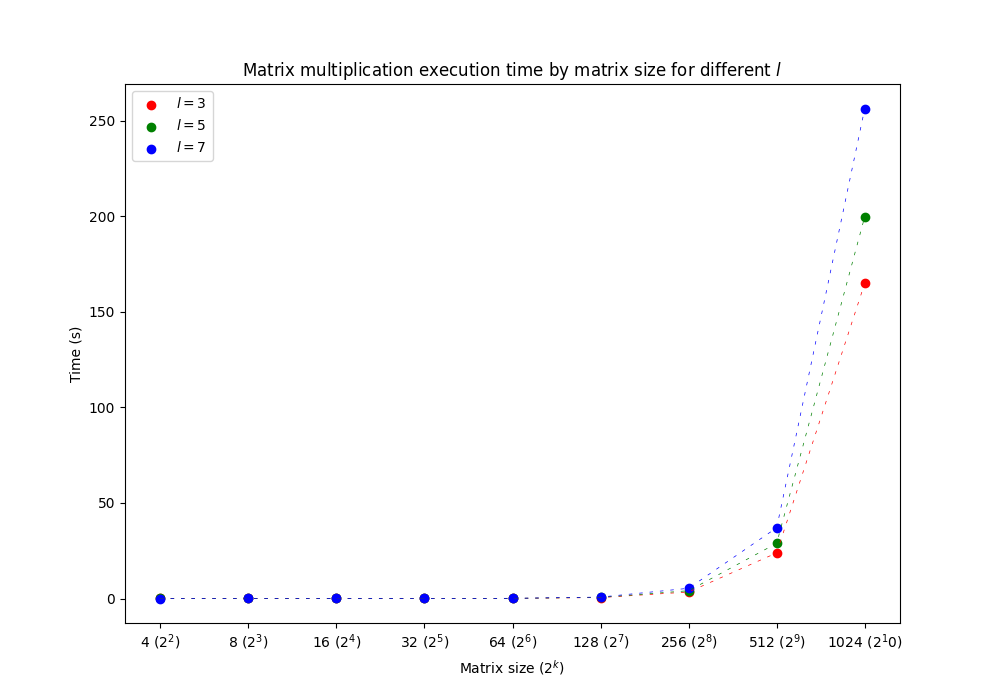
\includegraphics[scale=0.35]{linear_time_scatter_plot.png}
  \caption{Wykres czasu mnożenia macierzy w zależności od rozmiaru macierzy.}
\end{figure}

\begin{figure}[h]
  \centering
  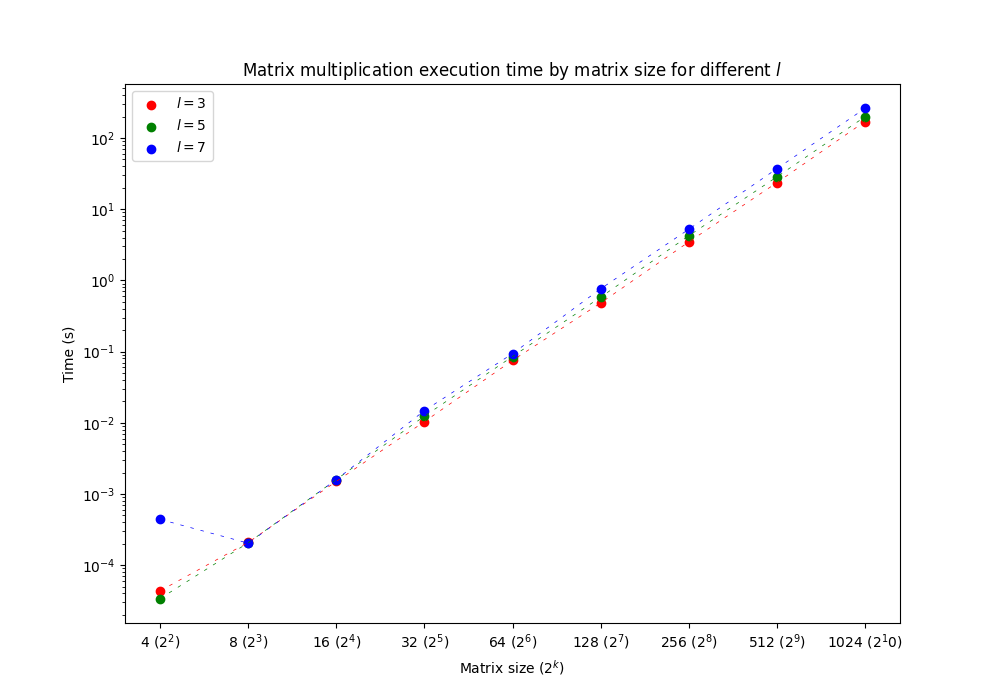
\includegraphics[scale=0.35]{log_time_scatter_plot.png}
  \caption{Wykres czasu w skali logarytmicznej w zależności od rozmiaru macierzy}
\end{figure}

\subsection{Wykresy liczebności operacji zmiennoprzecinkowych dla różnych $l$}

\begin{figure}
  \centering
  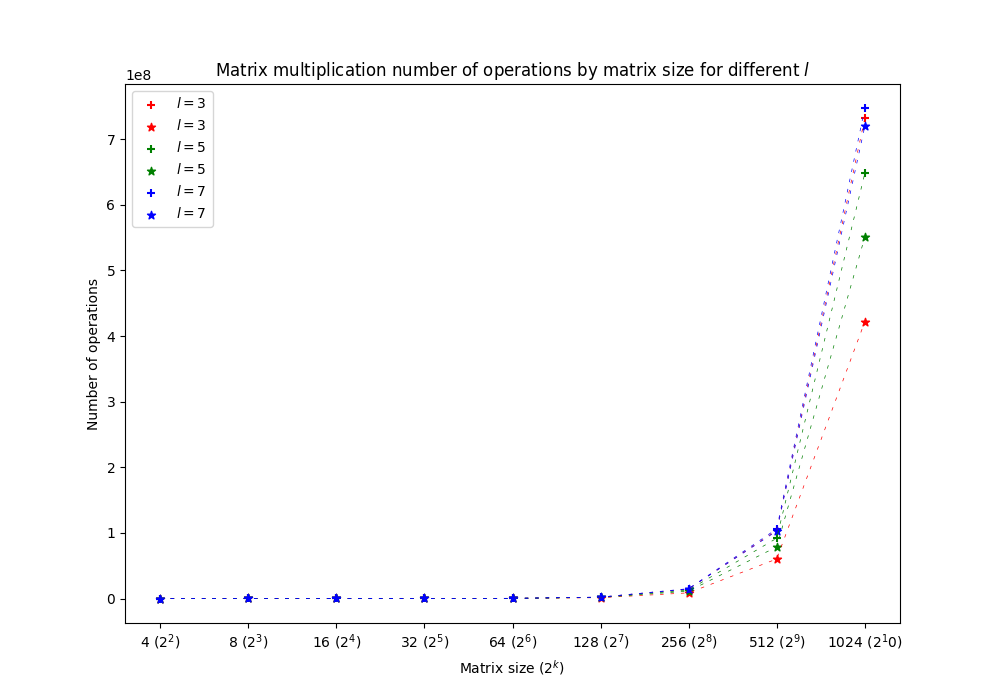
\includegraphics[width=\linewidth]{linear_operations_counter_scatter_plot.png}
  \caption{Wykres liczebności operacji zmiennoprzecinkowych w zależności od rozmiaru macierzy}
\end{figure}

\begin{figure}
  \centering
  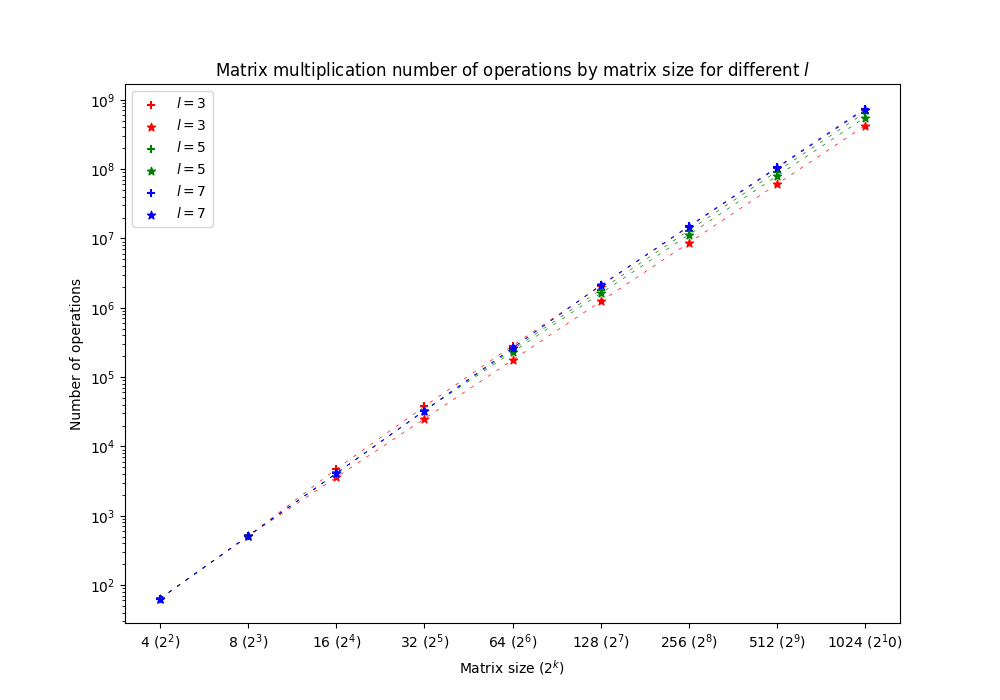
\includegraphics[width=\linewidth]{log_operations_counter_scatter_plot.png}
  \caption{Wykres liczebności operacji zmiennoprzecinkowych w zależności od rozmiaru macierzy}
\end{figure}

\end{document}
